\documentclass[twocolumn]{article}
\usepackage{graphicx}
\usepackage{float}
\usepackage{placeins}

\usepackage{geometry}
\geometry{margin=1in}
\usepackage{abstract}
\renewcommand{\abstractnamefont}{\normalfont\Large\bfseries} % Abstract title font
\renewcommand{\abstracttextfont}{\normalfont} % Abstract text font
\usepackage{titlesec}
\usepackage{hyperref}

\title{Multi-Splat Representations: Segmentation and Object Manipulation in Gaussian Splatting}
\author{Bavo Verstraeten\\
	Promotors: Prof. dr. Peter Lambert, Prof. dr. ir. Glenn Van Wallendael}

\begin{document}
	\pagenumbering{gobble}
	
\twocolumn[
\maketitle
\begin{onecolabstract}
	\noindent
Gaussian splatting is a novel technique for real-time rendering of complex scenes. This thesis improves the usability and accuracy of Gaussian splats in the Unity engine by extending an existing open-source Unity extension. Two key challenges are addressed. First, the original Unity extension performs per-GameObject sorting and rendering of splats, leading to visual artifacts when multiple splat objects overlap. To resolve this, the existing rendering pipeline was adapted to perform global per-splat sorting, enabling correct depth ordering across all splats in the scene. Second, the preparation of splats for animation in Unity traditionally requires manual and error-prone segmentation. To facilitate this process, a semi-automatic segmentation pipeline was developed by combining the tools SAM, SAM2, and SAGD. This approach automates much of the segmentation process, while retaining user control for refinement and correction, ultimately producing hierarchical GameObjects from splat data. These contributions enhance both rendering fidelity and workflow usability, advancing the integration of Gaussian splatting into real-time interactive applications.
\end{onecolabstract}
\vspace{1cm}
]
	
	\section{Introduction}
In recent years, the field of real-time 3D rendering has experienced a shift from traditional geometry-based representations to point-based methods that better capture complex scene details. Among these, Gaussian splatting \cite{OriginalSplatting} has emerged as a compelling alternative, offering the ability to render photorealistic scenes in real-time by representing surfaces as a collection of spatially distributed Gaussians. Unlike neural-network-based approaches such as Neural Radiance Fields (NeRF) \cite{Nerf}, Gaussian splatting bypasses the need for expensive network queries, making it well-suited for interactive applications where performance is critical.
\\\\
However, adapting Gaussian splatting techniques for use in real-time engines like Unity introduces unique challenges. The existing open-source implementation \cite{Aras}, while functional, reveals limitations when applied to dynamic or interactive environments. Notably, issues with rendering depth and manual segmentation workflows hamper the seamless integration of this promising technique into common production pipelines.
\\\\
This work explores these challenges in depth, identifying key bottlenecks and proposing concrete solutions that enhance both the visual fidelity and usability of Gaussian splats in Unity. By focusing on both the rendering architecture and the segmentation process, the study aims to bridge the gap between academic advances in point-based rendering and their practical deployment in real-time interactive systems.

	\section{Methodology}
	\subsection{Global Per-Splat Sorting}
The Unity extension applies per-GameObject sorting, meaning that for any two GameObjects, one is always rendered completely in front of the other. This approach works for simple scenes but leads to rendering artifacts in more complex cases.
\\\\
To address this, the renderer was modified to implement global per-splat sorting. Instead of assigning each GameObject its own graphics buffer for processed splat data, a single global graphics buffer was introduced. Each object's compute shader writes directly into this buffer, ensuring splat data from all objects is combined efficiently. Once the global buffer is populated, it is sorted and rendered based on the true depth of each splat, producing correct and consistent visual results without introducing unnecessary complexity.


	
	\subsection{Segmentation Pipeline}
The Unity extension provides a built-in tool for manually isolating segments of a Gaussian Splat. However, this method becomes increasingly cumbersome and inefficient when dealing with large or complex segments, making automated assistance highly desirable. Automatic segmentation typically begins with an image mask, and among the various methods explored in the literature, SAGD \cite{SAGD} emerged as particularly suitable. SAGD introduces Gaussian decomposition, a process that splits splats along the mask boundary, thereby smoothing segment edges and addressing the problem of large, chaotic interior splats common in Gaussian Splat models.
\\\\
SAGD faces challenges when converting a 2D image mask into an accurate 3D splat mask. To overcome these limitations, SAM \cite{SAM} and SAM2 \cite{SAM2} were integrated into the segmentation pipeline. SAM2 is capable of video segmentation, allowing masks to be generated from multiple angles when continuous training data is available. SAM, while focused on image segmentation, offers a versatile suite of tools that complement both SAM2 and SAGD.
\\\\
Together, these three tools—SAM, SAM2, and SAGD—form a flexible segmentation pipeline capable of supporting multiple levels of automation. The user can choose to provide hierarchical prompts for precise segmentation, rely on automatic hierarchy calculation to reduce manual input, or allow the system to perform full segmentation without any user intervention.
	
	\section{Results}
	Figure~\ref{fig:render} demonstrates the rendering artifacts caused by per-GameObject sorting and the improvements achieved with global per-splat sorting. The bulldozer’s arm, which is implemented as a separate GameObject, poses a challenge for per-GameObject sorting. In the left image, the pumps on the arm are not visible. In the right image, a part of the front section of the bulldozer has disappeared. The bottom image shows the corrected rendering achieved with global per-splat sorting, where each splat’s depth is evaluated globally, resolving these artifacts and preserving the model's visual coherence.
	\begin{figure}[h!]
		\centering
		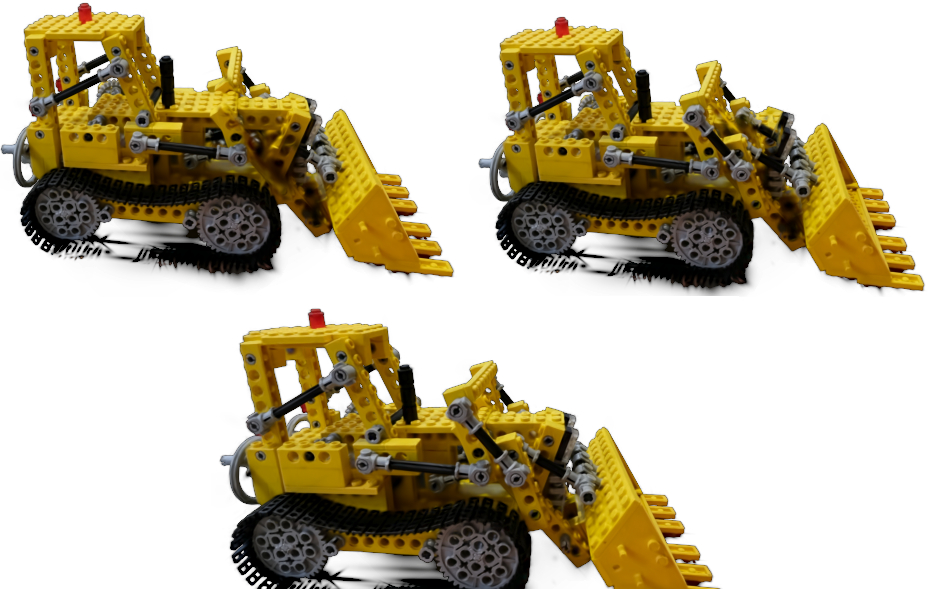
\includegraphics[width=0.5\textwidth]{Images/Untitled.png}
		\caption{Incorrect rendering due to per-GameObject sorting (left, right). Correct rendering with global per-splat sorting (bottom).}
		\label{fig:render}
	\end{figure}
	\FloatBarrier
	\noindent
	Figure~\ref{fig:trucks} illustrates the segmentation performance of the developed pipeline, which integrates three distinct algorithms to provide varying levels of automation and control. The top image demonstrates fully automatic segmentation, where the truck model is decomposed into multiple segments without any user input. The right image showcases the semi-automatic approach, where a single positive point prompt is used to simultaneously isolate the truck from the surrounding scene and extract the wooden platform from the truck itself. This method provides minimal input while offering limited control over the output. Although not depicted, the pipeline also supports a semi-automatic method with full user guidance, where the user can define hierarchical prompts and steer the segmentation process as desired, achieving precise extraction of any combination of segments within the scene. Although the results are not without imperfections, these algorithms are not in competition; rather, they complement one another and each excels under specific conditions.
	\begin{figure}[h!]
		\centering
		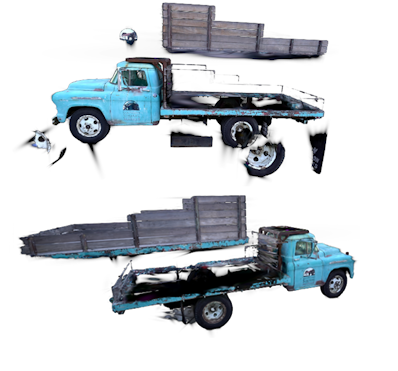
\includegraphics[width=0.5\textwidth]{Images/trucks.png}
		\caption{Segmentation of a truck model: fully automatic (top) and semi-automatic with a single prompt (bottom).}
		\label{fig:trucks}
	\end{figure}
	\FloatBarrier
	\noindent
	\section{Discussion}
This work addresses a significant challenge in integrating Gaussian splats within the Unity engine by resolving a critical rendering error related to the sorting of splats. By introducing a global sorting mechanism, the rendering pipeline’s correctness is notably improved, ensuring that splat-based scenes render without artifacts, even in complex interactive environments. The improved pipeline enhances the utility of the existing open-source Unity extension, providing a more robust tool for both researchers and developers to experiment with and manipulate splats. This advancement is expected to benefit a wide range of real-time rendering applications and further adoption of Gaussian splatting techniques.
\\\\
A key contribution of this thesis is the novel combination of Gaussian decomposition with more consistent and reliable mask generation across multiple views. This enhancement extends the applicability of decomposition-based segmentation to increasingly complex scenes. Furthermore, the introduction of multiple levels of automation within the segmentation workflow improves usability and provides flexible solutions for a variety of segmentation tasks.
\\\\
Nonetheless, several limitations remain. The fully automated segmentation algorithm occasionally generates nonsensical segments, particularly in scenes with high complexity or occlusion. Additionally, applying Gaussian decomposition to large and intricate scenes has resulted in memory allocation failures, indicating scalability constraints. Furthermore, the reliance on a continuous training video for SAM2 introduces a limitation on the types of models that can be processed, reducing the system’s general applicability.
\\Future research directions are clear. One promising avenue is the simulation of a moving camera within Unity to generate continuous video input for SAM2. Improvements in mask combination strategies could also yield more reliable and precise segmentations. Moreover, incorporating information about the three-dimensional positions and structures of splats—currently underutilized in this paper—may enhance segmentation quality and stability, especially in dense or occluded scenes.
	\section{Conclusion}
By addressing critical limitations in both rendering and segmentation, this work significantly advances the practical integration of Gaussian splatting into real-time applications. The developed solutions not only improve visual fidelity and workflow efficiency in Unity but also pave the way for future research in high-fidelity, point-based scene representations and their applications in interactive systems. These contributions mark a meaningful step toward realizing the full potential of Gaussian splatting in complex, dynamic environments.
\bibliographystyle{IEEEtran}
\bibliography{references}

\end{document}
